L'analyse d'un logiciel malveillant a pour but de comprendre ses mécanismes internes : selon les logiciels il peut, entre autres, s'agir des techniques d'attaque, de communication avec d'autres instances du programme ou l'attaquant, de clés de chiffrement utilisées. Le programmeur a donc intérêt à protéger son logiciel contre l'analyse. Son but est de la rendre plus compliquée, nécessitant plus de ressources en temps ou en argent de la part de l'analyste.

De nombreuses techniques de protection sont applicables à un programme binaire pour rendre son analyse plus compliquée. Certaines rendent le code plus difficile à comprendre en ajoutant par exemple du code inutile. Une autre technique consiste à modifier le programme au cours de son exécution afin que le code réellement utile du binaire ne soit pas lisible à première vue : on parle alors d'auto-modification.

Un auteur de programmes malveillants peut produire dans un premier temps son programme sans protection puis utiliser un logiciel de protection qui produit un binaire sémantiquement équivalent mais qui est rendu plus difficile à analyser. En pratique l'exécutable final, protégé, combine plusieurs techniques d'obscurcissement dont des techniques d'auto-modification.

Dans ce chapitre nous chercherons rapidement a comprendre les difficultés rencontrées pour quiconque cherche à protéger son programme contre l'analyse. Dans un second temps nous nous intéresserons aux protections rencontrées lors de l'analyse de logiciels malveillants et en particulier aux problèmes liés au chevauchement de code assembleur et à l'auto-modification.

% Nous décrivons maintenant plusieurs techniques d'obscurcissement statiques ainsi que l'auto-modification.

% $\mathcal{T}$

\section{Théorie de l'obscurcissement}
Collberg et Nagra \cite{nagra2009surreptitious} définissent plusieurs propriétés souhaitables pour une protection logicielle, nous reprenons ici quelques uns de leurs arguments. La première propriété est que le programme protégé soit équivalent en terme de sorties que le programme d'origine.
Une protection, ou obscurcissement, d'un programme P est une transformation $\mathcal{T}$ telle que le programme $\mathcal{T}(P)$ a le même comportement que P : quelle que soit l'entrée I de P, $\mathcal{T}(P)(I)=P(I)$.
On souhaite également ne pas affecter de manière importante les performances du programme, que ce soit en termes de temps d'exécution ou de taille des binaires.

Afin d'évaluer l'efficacité des protections il est nécessaire de définir les actifs que l'on cherche à protéger. 
Il peut s'agir de quelques algorithmes centraux au programme, de clé de chiffrement, du nom des fonctions et des variables utilisées, etc.
Il est également utile de masquer l'utilisation de techniques de protection qui pourraient attirer l'attention lors d'une analyse antivirale. De même si l'analyste se doute que le binaire emploi des protections, il n'est pas souhaitable qu'il lui soit aisé d'identifier quelles méthodes sont employées. Ainsi dans les modifications apportées au programme il est préférable que le programme final ressemble à un programme qui aurait pu être compilé, par exemple en évitant d'utiliser des instructions exotiques rarement utilisées en général.


En pratique un auteur de logiciel malveillant masque les symboles utiles à l'analyse tels le nom des fonctions à la compilation. Il est utile que le vecteur de propagation réussisse à masquer qu'il est protégé, s'il l'est, pour éviter une détection prématurée par un antivirus. 
% La charge finale et les éventuels mécanismes de communication sont eux protégés contre l'analyse.\todo{cite}

\section{Exemples d'obscurcissement}
De nombreuses techniques d'obscurcissement sont utilisées en pratique, nous en donnons quelques exemples ici.

\paragraph{Insertion de code mort.}
Insérer du code non atteignable (ou code mort) peut forcer un désassembleur par parcours linéaire à se désaligner avec le code réellement exécuté et à favoriser le code mort au détriment du code légitime.
L'exemple donné en figure \ref{fig:junk_right} montre de l'assembleur avec deux octets de données placés à la suite d'une instruction \jmp. Ces deux octets aux adresses $0x08048062$ et $0x08048063$ ne sont pas atteignables. Pourtant un désassembleur linéaire (Figure \ref{fig:junk_fooled}) chercherait à les désassembler et serait alors incapable de voir une partie des instructions réellement exécutées.

\begin{figure}
\begin{lstlisting}[language={[x86masm]Assembler}, escapechar=~]
jmp suite
db    0a 05	; ~Octets non atteignables~
suite:
cmp ecx, 0x2
je 0x8048069
mov ebx, 0x2 ;  0x00000002
\end{lstlisting}
\caption{Insertion de code mort dans du code légitime}
\label{fig:junk_right}
\end{figure}


\begin{figure}
\begin{lstlisting}[language={[x86masm]Assembler}, escapechar=~]
08048060    eb 02               jmp 0x8048064
08048062    0a 05 83 f9 02 74   or al, [0x7402f983]
08048068    00 bb 02 00 00 00   add [ebx+0x2], bh
\end{lstlisting}
\caption{L'insertion de code mort dupe facilement un désassemblage par parcours linéaire}
\label{fig:junk_fooled}
\end{figure}

\FloatBarrier

\paragraph{Appels de fonctions sans retour.}
L'utilisation d'un contrôle de flot non standard peut forcer un désassembleur par parcours récursif à explorer du code non atteignable. 
Le comportement par défaut de l'instruction \call\ à une adresse $a$ et de taille $n$ est d'empiler l'adresse de retour $a+n$ puis de sauter vers la première adresse de la fonction appelée.
L'instruction \ret\ placée à la fin de la fonction appelée dépile la première valeur de la pile et provoque un saut vers celle-ci.

Normalement la valeur dépilée lors du \ret\ est $a+n$ afin que le flot d'exécution revienne à la fonction appelant.
Ainsi un désassembleur récursif désassemble à partir de la cible du \call\ ainsi que de l'adresse de retour.

Une technique classique d'obscurcissement \cite{LD03}\cite{PMA} consiste à combiner l'empilement d'une adresse (\push\ $a$) et l'instruction \ret. Ces deux instructions provoquent un saut vers l'adresse $a$ sans possibilité de revenir à l'instruction suivant le \call. La transformation consiste alors à remplacer des instructions \jmp\ par la séquence \push\ puis \ret\ puisque les deux suites d'instructions suivantes sont équivalentes.
\begin{center}
\begin{tabular}{c|c}
\push\ \adr{a} & \jmp\ \adr{a}\\
\ret &
\end{tabular}
\end{center}

\paragraph{Prédicats opaques.}
% À l'instar de son comportement avec une instruction \call, 
Lorsqu'un désassembleur récursif rencontre une instruction de saut conditionnel comme \je, qui provoque un saut si les deux valeurs comparées sont égales, il cherche à désassembler à la fois la cible potentielle du saut comme l'instruction suivante, qui sera exécutée si la condition n'est pas remplie.
Une autre technique courante d'obscurcissement \cite{MKK07} consiste à utiliser comme condition du saut une relation que le programmeur sait toujours vraie ou fausse. De cette manière il prédit qu'une seule des deux branches est atteignable alors qu'un désassembleur va parcourir également la branche inutile.
Une telle condition est appelée un prédicat opaque et peut être implémentée par des relations d'arithmétique. Par exemple en appliquant le petit théorème de Fermat \cite{fermat} : quel que soit l'entier e, $e^3\ =\ e\ mod\ 3$.
Le programmeur sait que l'égalité est toujours vérifiée mais un analyseur statique ne pourra pas le déterminer aisément.

\itodo{Applatissement de graphe de flot de contrôle.}

\section{Chevauchement de code}
On a vu que la taille d'une instruction assembleur varie de un à 15 octets \done{15 dans intel2 chercher 15}.
De plus rien n'empêche que la cible d'un saut soit une adresse se trouvant être au milieu d'une autre instruction.
Ainsi on parle de chevauchement de code lorsque deux instructions (ou plus) à des adresses différentes sont codées sur des adresses communes. Si une instruction à l'adresse \adr{a} de taille $k\geq 2$ est atteignable, il peut y avoir une autre instruction valide et atteignable à l'adresse \adr{a+1} et ces deux instructions se chevauchent.

Il est à noter que, comme indiqué par Sikorski et Honig \cite{PMA}, il n'y a dans ce cas aucun désassemblage sous forme de liste d'instructions assembleur qui soit correct puisqu'une telle liste devra choisir entre l'instruction à l'adresse \adr{a} et celle à l'adresse \adr{a+1} alors qu'elles sont toutes les deux valides et atteignables. Une solution pour écrire un tel code assembleur est de mettre la première instruction en temps qu'instruction classique tandis que la deuxième sera présente sous forme d'octets codés en dur dans le fichier assembleur.

\subsection{Exemples de chevauchement}

\paragraph{Dans \telock.}
Le code de la figure \ref{fig:telock_obf_disas} est extrait d'un programme protégé par \telock\ désassemblé à l'aide d'un parcours récursif à partir de l'adresse \adr{01006e7a}. Il y a une instruction \texttt{jmp +1} à l'adresse \adr{01006e7d} et codée sur les deux octets \texttt{eb ff}, qui saute vers l'adresse \adr{01006e7d+1} où est présenté l'instruction \texttt{dec ecx}, codée sur \texttt{ff c9} et qui partage donc l'octet \texttt{ff} à l'adresse \adr{01006e7d+1} avec l'instruction \jmp.

Le code assembleur permettant d'être assemblé en ces octets est donné figure \ref{fig:telock_obf_asm} : la première instruction \jmp\ peut être présente dans le code tandis que l'instruction \dec\ la chevauchant est codée en dur grâce à l'octet \texttt{c9}.

\begin{figure}
% \scriptsize
% 0x01006e73    00 0c 0b        add [ebx+ecx], cl
% 0x01006e76    80 34 0b 67     xor byte [ebx+ecx], 0x67
Octets à désassembler : \texttt{fe 04 0b eb ff c9 7f e6 8b c1}
\begin{lstlisting}[language={[x86masm]Assembler}, escapechar=~]
01006e7a    fe 04 0b        inc byte [ebx+ecx]
01006e7d    eb ff           jmp +1
01006e7e       ff c9        dec ecx
01006e80    7f e6           jg 01006e68
01006e82    8b c1           mov eax, ecx
\end{lstlisting}
% \end{framed}
\caption{Désassemblage récursif de \telock}
\label{fig:telock_obf_disas}
\end{figure}

\begin{figure}
% \scriptsize
% 0x01006e73    00 0c 0b        add [ebx+ecx], cl
% 0x01006e76    80 34 0b 67     xor byte [ebx+ecx], 0x67
\begin{lstlisting}[language={[x86masm]Assembler}, escapechar=~]
inc byte [ebx+ecx]
jmp +1
db c9 		; ~l'ajout de l'octet \texttt{c9} complète l'instruction \texttt{dec ecx}~
jg 01006e68
mov eax, ecx
\end{lstlisting}
% \end{framed}
\caption{Code assembleur du chevauchement de \telock}
\label{fig:telock_obf_asm}
\end{figure}


Le graphe de flot de contrôle correct pour ce code est donné sur la figure \ref{fig:telock_cfg}. Le sommet orange est la première instruction et les lignes en pointillés reliant deux sommets marquent un chevauchement entre les instructions de ces sommets.

\begin{figure}
\begin{center}
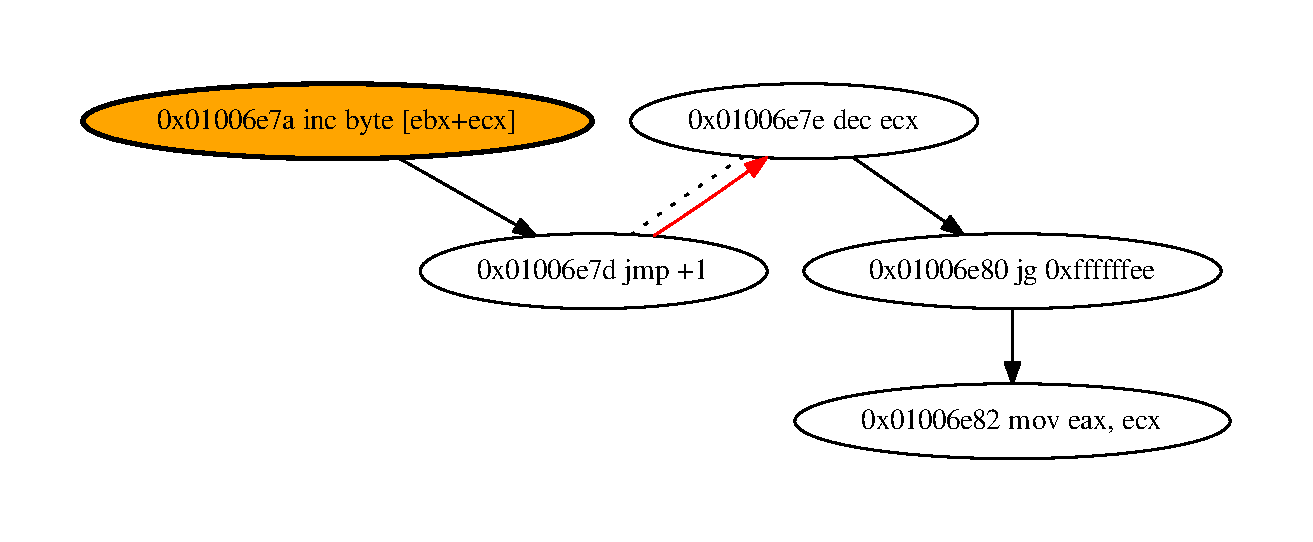
\includegraphics[width=0.8\textwidth]{supports/disasm/telock/telock.pdf}
\end{center}
\caption{Graphe de flot de contrôle de \telock}
\label{fig:telock_cfg}
\end{figure}

% \begin{figure}
% \begin{center}
% \begin{tabular}{|l|c|c|c|c|c|}
% \hline
% Addresses & 0x01006e7d & 0x01006e7e & 0x01006e7f & 0x01006e80 & 0x01006e81\\
% \hline
% Bytes & eb & ff & c9 & 7f & e6\\
% \hline
% Layer 1 @0x01006e7d & \multicolumn{2}{c|}{jmp +1} & \cellcolor[gray]{0.0} & \multicolumn{2}{c|}{jg 0x1006e68}\\
% \hline
% Layer 2 @0x01006e7e & \cellcolor[gray]{0.0} & \multicolumn{2}{c|}{dec ecx} & \multicolumn{2}{c|}{\cellcolor[gray]{0.0}} \\
%  \hline
% % \\
% \end{tabular}
% \end{center}
% \caption{Layers of a subset of the TELock code segment}
% \label{fig:telock-layers-recursive}
% \end{figure}
% 
% \begin{figure}
% \begin{center}
% \begin{tabular}{|l|c|c|c|c|c|c|c|c|c|c|}
% \hline
% Addresses & 0xf2 & 0xf3 & ... & 0xf9 & 0xfa & 0xfb & 0xfc & 0xfd & 0xfe & 0xff\\
% \hline
% Bytes & 79 & 07 & ... & 47 & b9 & 57 & 48 & f2 & ae & 55\\
% \hline
% Layer 1 @0xf2 & \multicolumn{2}{c|}{jns +9 (0xfb)} & ... & inc edi & \multicolumn{5}{c|}{mov ecx, aef24857} & push ebp\\
% \hline
% Layer 2 @0xfb & \multicolumn{5}{c|}{\cellcolor[gray]{0.0}} & push edi & dec eax & \multicolumn{2}{c|}{repne scasb} & \cellcolor[gray]{0.0}\\
% \hline
% % \\
% \end{tabular}
% \end{center}
% \caption{Layers of a subset of the UPX code segment}
% \label{fig:upx-layers-recursive}
% \end{figure}

\paragraph{Dans UPX.}
UPX \cite{UPX} cherche à optimiser la taille du binaire protégé.
La procédure d'exécution du binaire protégé utilise un saut conditionnel pour séparer le contrôle de flot en deux blocs se chevauchants et finissant sur un bloc où ils se réalignent.
\todo{expliquer les deux branches, rapidement en quoi elles sont utiles}
\begin{figure}
% \scriptsize
Octets à désassembler : \texttt{89 f9 79 07 0f b7 07 47 50 47 b9 57 48 f2 ae 55}
\begin{lstlisting}[language={[x86masm]Assembler}, escapechar=~]
    010059f0    89 f9            mov ecx, edi
,=< 010059f2    79 07            jns +9
|   010059f4    0f b7 07         movzx eax, word [edi]
|   010059f7    47               inc edi
|   010059f8    50               push eax
|   010059f9    47               inc edi
|   010059fa    b9 57 48 f2 ae   mov ecx, aef24857
`->   010059fb     57            push edi
      010059fc        48         dec eax
      010059fd           f2 ae   repne scasb
    010059ff    55               push ebp
\end{lstlisting}
% \end{framed}
\caption{Chevauchement de code dans UPX\label{fig:upx_obf_disas}}
\end{figure}
Le graphe de flot de contrôle pour ce chevauchement est donné en figure \ref{fig:upx_cfg}.

\begin{figure}
\begin{center}
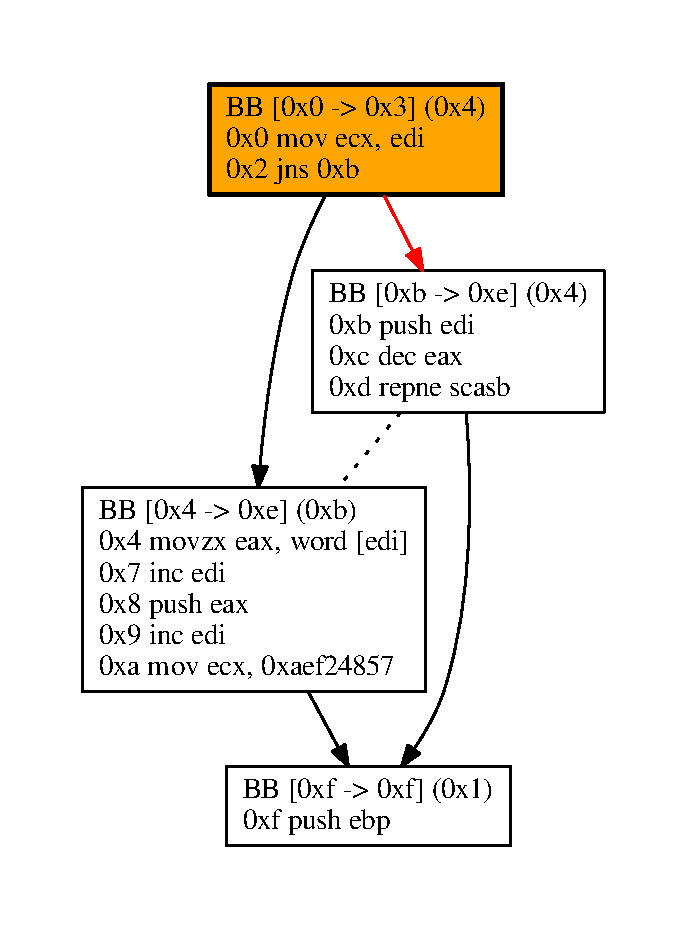
\includegraphics[width=0.4\textwidth]{supports/disasm/upx/upx.pdf}
\end{center}
\caption{Graphe de flot de contrôle de l'échantillon d'UPX}
\label{fig:upx_cfg}
\end{figure}

\FloatBarrier

\paragraph{Cacher une séquence de code de taille arbitraire.}
Jämthagen, Lantz et Hell \cite{JLH13} ont proposé un moyen d'inclure une longue séquence de code cachée au sein d'une séquence d'assembleur valide qui s'exécute sans provoquer d'erreur.

Une des possibilités est d'utiliser une instruction \nop\ avec préfixe qui se code sur neuf octets. La partie fixe (préfixe et opérande) est codée sur quatre octets (\texttt{66 0f 1f 84}) tandis que les cinq autres octets peuvent être choisis arbitrairement.
Ainsi chaque instruction \nop\ peut véhiculer 5 octets de code caché. Afin d'encoder une séquence de code dans une séquence de \nop\ il faut pouvoir utiliser les 4 octets fixes de l'instruction \nop\ suivante de manière utile ou non perturbante pour la séquence de code caché.
Une possibilité, si le registre \edx\ n'est pas utilisé dans la séquence à cacher, est de prendre \texttt{ba} pour dernier octet de chaque instruction \nop\ afin de former l'instruction \texttt{mov edx, 0x841f0f66} codée sur \texttt{ba 66 0f 1f 84}. On peut alors encoder n'importe quelles instructions de taille inférieure ou égale à quatre octets dans cette séquence de \nop.
Prenons la séquence suivante d'octets :
\begin{center}
\texttt{66 0f 1f 84} $\mathtt{x_1\ x_2\ x_3\ x_4}$ \texttt{ba 66 0f 1f 84} $\mathtt{y_1\ y_2\ y_3\ y_4}$ \texttt{ba 66 0f 1f 84} $\mathtt{z_1\ z_2\ z_3\ z_4}$.
\end{center}
Si on la désassemble linéairement à partir du premier octet il s'agit d'une séquence de trois \nop\ tandis que si on la désassemble à partir de $\mathtt{x_1}$, les instructions encodées dans les octets $\mathtt{x_i}$, $\mathtt{y_i}$ et $\mathtt{z_i}$ rentrent en considération :
\\

\begin{center}
\begin{tabular}{ll|ll}
\hline
 \multicolumn{2}{c|}{À partir du début} & \multicolumn{2}{c}{À partir de $x_1$} \\
\hline
 \texttt{66 0f 1f 84} $\mathtt{x_1\ x_2\ x_3\ x_4}$ \texttt{ba} & \nop & $\mathtt{x_1\ x_2\ x_3\ x_4}$ & ?\\
 \texttt{66 0f 1f 84} $\mathtt{y_1\ y_2\ y_3\ y_4}$ \texttt{ba} & \nop & \texttt{ba 66 0f 1f 84} & \texttt{mov edx, 0x841f0f66}\\
 \texttt{66 0f 1f 84} $\mathtt{z_1\ z_2\ z_3\ z_4}$ \texttt{ba} & \nop & $\mathtt{y_1\ y_2\ y_3\ y_4}$ & ?\\
  & & \texttt{ba 66 0f 1f 84} & \texttt{mov edx, 0x841f0f66}\\
    & & $\mathtt{z_1\ z_2\ z_3\ z_4}$ & ?\\
\end{tabular}
\end{center}

Les octets forment en fait deux chemin. L'un est exclusivement composé d'instructions \nop\ et est inoffensif : il s'agit du chemin d'exécution principal. Le second, le chemin d'exécution caché, débute à $\mathtt{x_1}$ et exécute le code que l'on souhaite dissimuler. En pratique le premier octet du chemin principal sera une cible valide et évidente du flot de contrôle tandis qu'il sera possible de sauter indirectement sur $\mathtt{x_1}$, par exemple avec un \texttt{jmp eax}. De cette manière le désassembleur est poussé à considérer le chemin principal sans examiner le chemin caché.

La limite est que les instructions cachées ne peuvent excéder une taille de 4 octets. Les auteurs expliquent cependant que beaucoup d'instructions \xq\ peuvent être séparées en plusieurs instructions plus petites, en utilisant par exemple des registres restreints comme \texttt{ax} ou \texttt{al} à la place d'\eax.


\subsection{État de l'art des contre-mesures}
\paragraph{Dans la littérature.}
Bien que le problème du chevauchement de code ne soit pas une technique d'obscurcissement récente et soit bien documentée \cite{PMA}, la littérature portant sur le désassemblage fait souvent l'hypothèse qu'un octet à une adresse spécifique ne peut être présent que dans une seule instruction \cite{KruegelRVV04}. Cette contrainte empêche de détecter tout chevauchement mais permet un désassemblage plus précis dans un binaire qui n'utilise pas cette technique de protection.
Nous verrons qu'en pratique l'utilisation du chevauchement de code est rare même dans un binaire protégé et proposerons une technique de désassemblage capable de détecter les cas de chevauchement.

Les auteurs de la techniques détaillée précédemment, permettant d'encoder une séquence de code cachée dans une séquence \cite{JLH13}, proposent de détecter la protection qu'ils exposent. L'idée est qu'il est improbable qu'une longue séquence d'octets représente une séquence valide de code. Si une telle séquence existe, c'est sûrement du code caché. Cette approche fonctionne pour la protection qu'ils exposent mais n'est pas applicable aux cas de \telock\ ou UPX par exemple car les séquences d'octets sur lesquels des instructions se chevauchent sont très courtes.

\paragraph{Désassembleurs disponibles.}
Les désassembleurs existants, qu'ils utilisent un parcours linéaire ou récursif, font également l'hypothèse que le code ne peut pas se chevaucher et ne parviennent pas à afficher un désassemblage cohérent dans le cas contraire.

Le désassemblage récursif de l'exemple de \telock\ avec IDA Pro (version 6.3) \cite{IDA} est le suivant :
\begin{lstlisting}[language={[x86masm]Assembler}, escapechar=~]
01006E7A     inc     byte ptr [ebx+ecx]
01006E7D     jmp     short near ptr loc_1006E7D+1
; ~Les octets suivants n'ont pas été désassemblés~
01006E7F     db 0C9h
01006E80     db  7Fh
01006E81     db 0E6h
01006E82     db  8Bh
01006E83     db 0C1h
\end{lstlisting}
Radare \cite{radare} effectue le désassemblage linéaire suivant :
\begin{lstlisting}[language={[x86masm]Assembler}, escapechar=~]
01006e7a    fe 04 0b     inc byte [ebx+ecx]
01006e7d    eb ff        jmp 6e7e
01006e7f    c9           leave
01006e80    7f e6        jg 6e68
01006e82    8b c1        mov eax, ecx
\end{lstlisting}
Ni l'un ni l'autre n'est capable de suivre le saut de l'instruction \jmp\ : la cible du saut a déjà été prise en compte comme faisant partie d'une autre instruction.

De même ni Radare ni IDA ne détectent le second chemin d'exécution dans l'extrait d'UPX et désassemblent cet extrait comme suit.
\begin{lstlisting}[language={[x86masm]Assembler}, escapechar=~]
010059f0    89 f9            mov ecx, edi
010059f2    79 07            jns 0x10059fb
010059f4    0f b7 07         movzx eax, word [edi]
010059f7    47               inc edi
010059f8    50               push eax
010059f9    47               inc edi
010059fa    b9 57 48 f2 ae   mov ecx, 0xaef24857
010059ff    55               push ebp
\end{lstlisting}

\section{Auto-modification}

% \begin{figure}
% \begin{center}
% \begin{tabular}{|l|l|l|}
% \hline
% Adresse & Octets & Instruction\\
% \hline
%  8048060  &  (...)         	& Pile -> RWX \\ 
%  804807c  &  bf 00 00 00 00         &  mov    edi, 0x0 \\
%  8048081  &  b8 91 80 04 08         &  mov    eax, 0x8048091 \\
%  8048086  &  66 c7 00 eb 00         &  mov    [eax], 0xeb \\
%  804808b  &  66 c7 40 01 07 00      &  mov    [eax+1], 0x7 \\
%  8048091  &  eb 0e                  &  jmp    80480a1 <edi3> \\
%  8048093  &  bf 01 00 00 00         &  mov    edi,0x1 \\
%  8048098  &  eb 0e                  &  jmp    80480a8 <fin> \\
%  804809a  &  bf 02 00 00 00         &  mov    edi,0x2 \\
%  804809f  &  eb 07                  &  jmp    80480a8 <fin> \\
%  80480a1  &  bf 03 00 00 00         &  mov    edi,0x3 \\
%  80480a6  &  eb 00                  &  jmp    80480a8 <fin> \\
%  80480a8  &  (...)		    &  Affiche edi \\
%  80480c3  &  (...)		    & Quitte \\
% \hline
% \end{tabular}
% \end{center}
% \caption{Exemple de code auto-modifiant}
% \label{fig:unevague_v0_code}
% \end{figure}

\begin{figure}
\begin{center}
\subfigure[Code assembleur]{
\begin{tabular}[b]{|l|l|l|}
\hline
Adresse & Octets & Instruction\\ 
\hline
 8048060  &  (...)         	& Pile -> RWX \\ 
 804807c  &  bf 00 00 00 00         &  mov    edi, 0x0 \\
 8048081  &  b8 91 80 04 08         &  mov    eax, 0x8048091 \\
 8048086  &  66 c7 00 eb 00         &  mov    [eax], 0xeb \\
 804808b  &  66 c7 40 01 07 00      &  mov    [eax+1], 0x7 \\
 8048091  &  eb 0e                  &  jmp    80480a1 <edi3> \\
 8048093  &  bf 01 00 00 00         &  mov    edi,0x1 \\
 8048098  &  eb 0e                  &  jmp    80480a8 <fin> \\
 804809a  &  bf 02 00 00 00         &  mov    edi,0x2 \\
 804809f  &  eb 07                  &  jmp    80480a8 <fin> \\
 80480a1  &  bf 03 00 00 00         &  mov    edi,0x3 \\
 80480a6  &  eb 00                  &  jmp    80480a8 <fin> \\
 80480a8  &  (...)		    &  Affiche edi \\
 80480c3  &  (...)		    & Quitte \\
\hline
\end{tabular}
\label{fig:unevague_v0_code}
}
\subfigure[Graphe de flot de contrôle]{
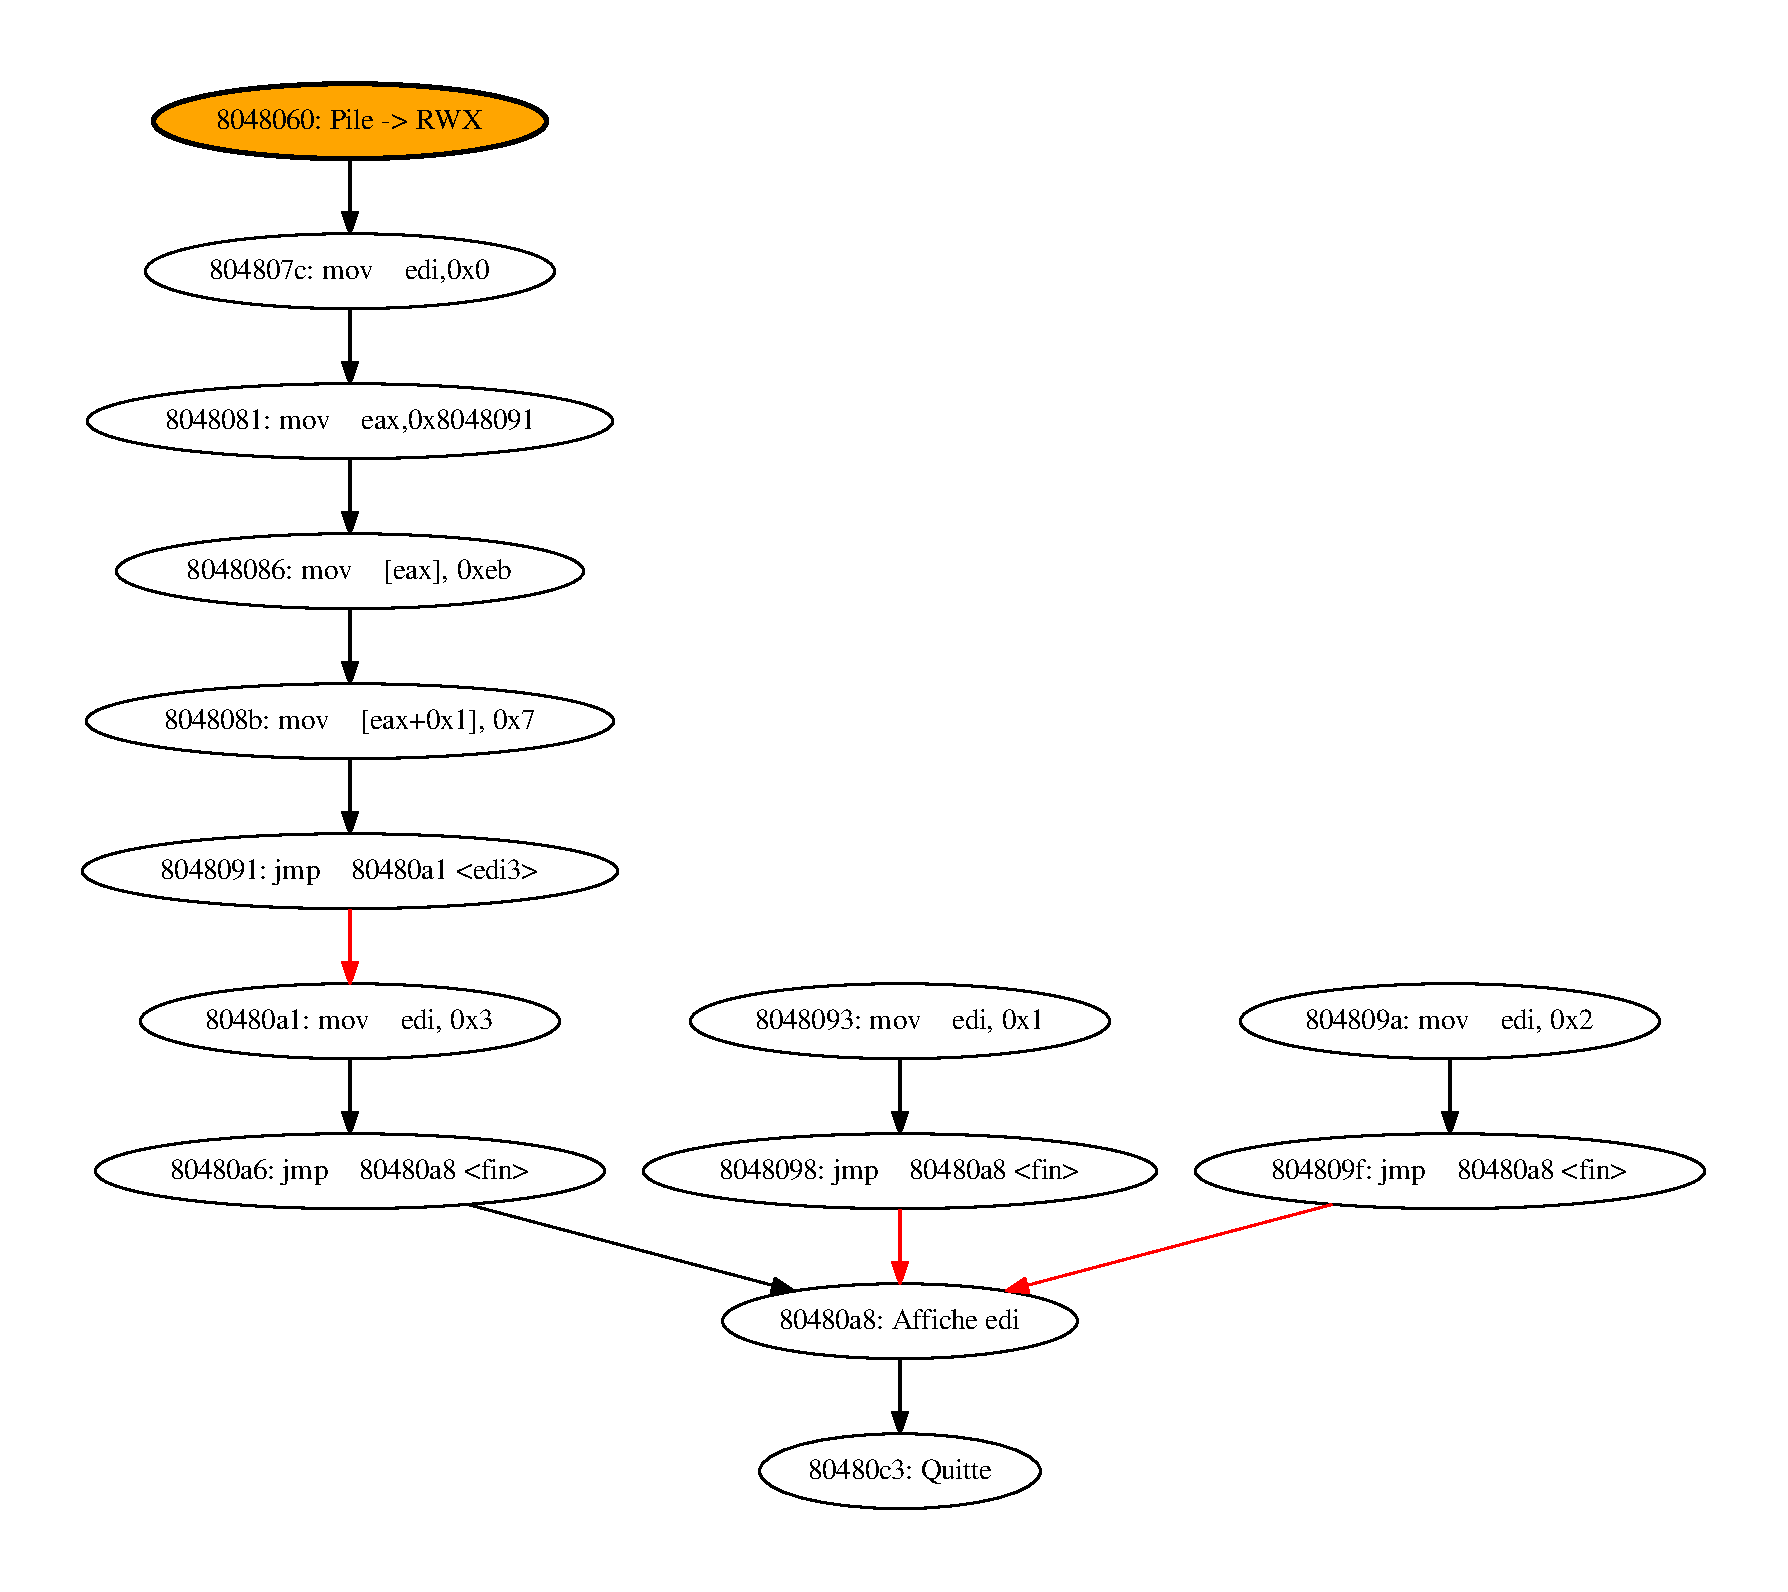
\includegraphics[width=1.0\textwidth]{supports/unevague/uv.pdf}
\label{fig:unevague_v0_cfg}
}
\end{center}
\ijym{détailler les ... (en annexe?)}
\ijym{fonction f, adresses f, f+1, f+3, ...}
\caption{Code assembleur auto-modifiant}
\label{fig:unevague_v0}
\end{figure}

Il a été expliqué dans la section \ref{section:assembleur} que, avec l'architecture de Harvard modifiée, le code n'est pas physiquement séparé des données lors de l'exécution sur une machine réelle.
Un programme auto-modifiant est simplement un programme utilisant cette propriété pour modifier le code assembleur le définissant au cours même de son exécution.
Ainsi on parle de comportement auto-modifiant lorsqu'une instruction du programme est codée sur au moins un octet qui a au préalable été modifié par ce programme.

En pratique les processeurs récents implémentent une protection, appelée bit NX ou W\textasciicircum X (prononcé ``W xor X''), permettant d'empêcher qu'une page mémoire puisse être à la fois écrite et exécutée lors de l'exécution du programme.
Cette protection a été ajoutée pour éviter des attaques résultant en l'exécution de code dans des données écrites par l'utilisateur du programme et non pour interdire l'auto-modification qui a des cas d'utilisation légitimes.
De ce fait l'activation ou non de la protection est spécifiée lors de la compilation et si un programme n'est pas protégé il lui suffit d'utiliser un appel système (\texttt{mprotect} sous linux) pour autoriser l'exécution de code sur la pile.

Prenons le programme de la figure \ref{fig:unevague_v0_code}. Ce programme commence par autoriser l'accès en écriture à la la section de code \ptext\ puis écrit sur la pile, modifie la valeur du registre \edi\ et termine par l'affichage de la valeur de \edi.
Si on ne prend pas en compte l'écriture sur la pile, il semble évident au vu du graphe de flot de contrôle (Figure \ref{fig:unevague_v0_cfg}), vu que la première instruction de saut provoque un saut vers l'instruction \texttt{mov edi,0x3} et que la seconde provoque l'affichage de \edi, que la valeur finale du registre est 3.
Pourtant les instructions \texttt{mov [eax],0xeb} et \texttt{mov [eax+1],0x07} aux l'adresse $0x8048086$ et $0x804808b$ remplacent le saut initial par un saut vers l'adresse $0x8048098$ où la valeur de \edi\ sera fixée à 2 avant l'affichage de celle-ci.


On constate ici que le programme se modifie au cours de son exécution et donc
\begin{itemize}
 \item On ne peut pas se contenter de la représentation d'origine du programme pour l'analyser.
 \item Le graphe de flot de contrôle initial peut être amené à évoluer au cours de l'exécution du programme.
\end{itemize}

\section{Logiciels malveillants et obscurcissement}
Un programmeur cherchant à protéger son binaire va se tourner vers les techniques d'obscurcissement dont nous avons donné quelques exemples ci-dessus. Puisque chacune des transformations a pour effet de rendre le programme plus difficile à comprendre, il n'y a souvent pas de limite au nombre de fois qu'il est possible d'itérer une technique de protection particulière. On peut alors chercher un compromis entre niveau de protection et complexité ajoutée au programme (en temps, en taille et en mémoire utilisée).

En pratique les auteurs des logiciels malveillants utilisent des logiciels existants pour protéger leurs binaires.
Ces logiciels de protection s'appliquent à l'ensemble du programme malveillant sans avoir à définir des atouts particuliers à protéger. On appelle ces programmes des empaqueteurs (\emph{packers}) : un empaqueteur prend un binaire en entrée et produit en sortie un binaire empaqueté, protégé. Une technique couramment utilisée est de cacher le binaire d'origine dans les données du binaire empaqueté, par exemple chiffré ou compressé (voir figure \ref{fig:packer}). Lors de l'exécution du binaire protégé une première phase consiste à restaurer le binaire d'origine en mémoire puis à effectuer un saut vers le point d'entrée du code restauré, provoquant ainsi l'exécution du binaire d'origine.

\begin{figure}
\begin{center}
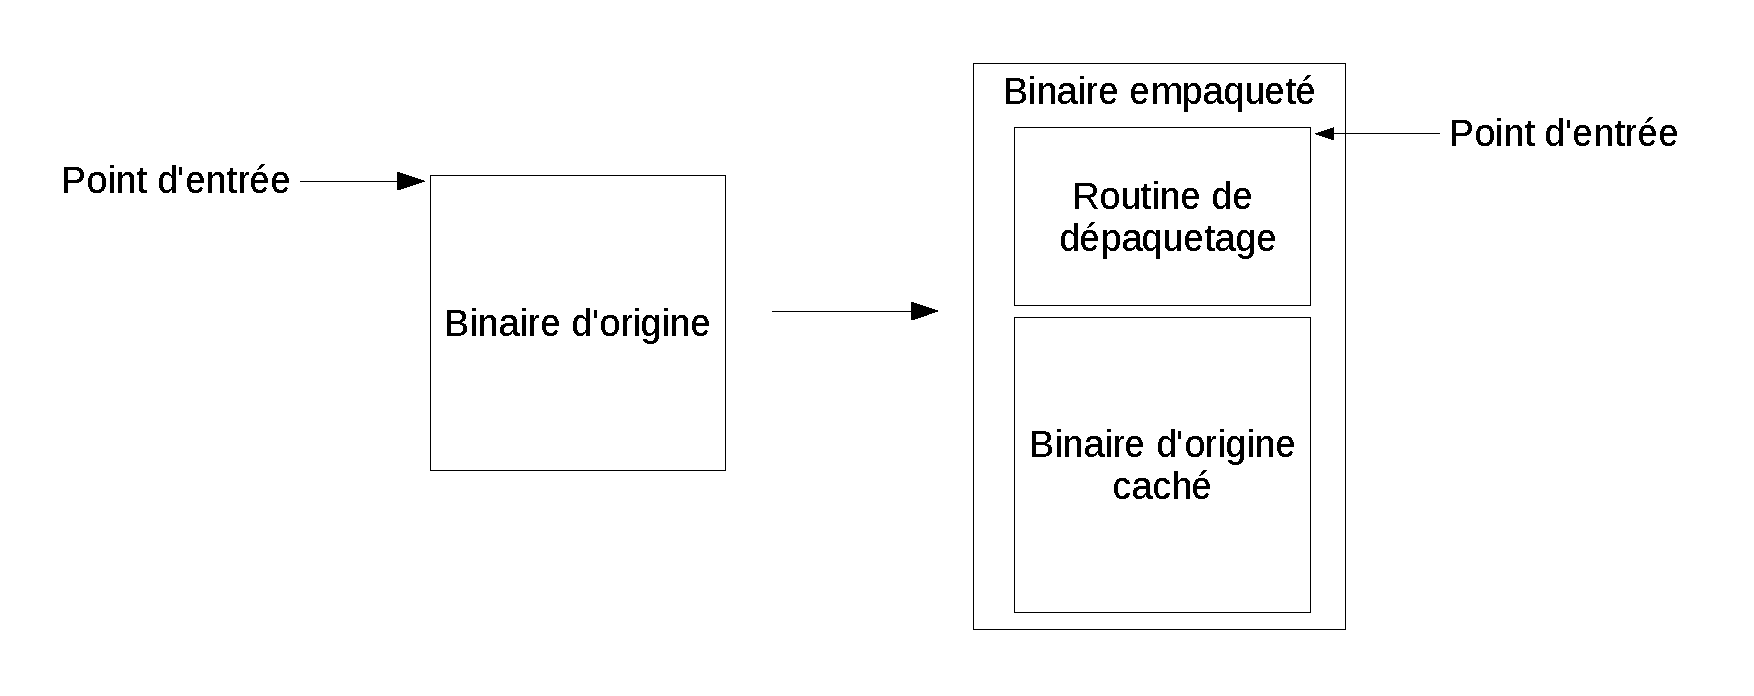
\includegraphics[width=1.0\textwidth]{supports/packers/packers.pdf}
\end{center}
\caption{Empaquetage d'un binaire}
\label{fig:packer}
\end{figure}

L'empaqueteur libre UPX \cite{UPX} est un cas typique du schéma précédent. Il compresse le binaire d'origine et le restaure à l'exécution. Ainsi il est plutôt conçu pour optimiser la taille du binaire paqueté et non pour l'obscurcir. La transformation utilisée étant réversible, l'empaqueteur permet également de récupérer le programme binaire d'origine sans l'exécuter. Il est cela dit parfois utilisé par des auteurs de logiciels malveillants sous une forme modifiée ne permettant plus de le dépaqueter automatiquement.


\section{Conclusion}
Cette thèse s'intéresse particulièrement à l'analyse des programmes écrits en assembleur \xq\ et \xs. Ces programmes ont en général été compilés à partir d'un langage de haut niveau puis ont été modifiés à l'aide d'un logiciel de protection. Les binaires que l'on étudie sont donc protégés avec des techniques statiques comme auto-modifiantes. Notre travail consiste alors à chercher à désassembler correctement ces programmes dans le but de faciliter leur analyse.

Les chapitres suivants détailleront plusieurs techniques d'analyse que nous avons appliquées. Nous nous intéresserons d'abord à l'aspect auto-modifiant des programmes et verrons comment l'analyse dynamique peut être utilisée pour reconstruire un modèle pour le programme auto-modifiant. Dans un second temps nous introduirons des techniques d'analyse statiques pour chercher à recomposer le maximum de code assembleur du programme et contourner d'autres méthodes de protection comme le chevauchement de code.